It is important to remark some StreamGen features that explain why the StreamGen language presented in this document slightly differs from the language of the four operators defined in \cite{privacypoliciesarticle}. StreamGen adds each new UML element at the end of the packaged elements of the UML file. Then, after using Acceleo, this could reach a Flink code which is not ordered and, then, a Flink code with errors. This happens only if the privacy language is based on privacy operators whose metaclass is a class as it is the case presented in \cite{privacypoliciesarticle}. Because of this, a research has been made in order to reach ordered Flink codes and the StreamGen language developed in this document is based on information flow metaclass.

\section{Privacy Policy Language}

StreamGen uses its own language in order to develop DIA. In this document, StreamGen language has been expanded in order to allow users to protect the streams with privacy policies. This expansion consists of a new data stream stereotype in order to specify which streams are protected and with which privacy policy type. Moreover, the sources that generate the Static Context Variables (SCV) and the rules written by the users are also added to the StreamGen language. SCV are going to be possibly supplied by different sources whilst privacy policies will be supplied only by one data source type. This sources are going to be inserted in a package which represents the external sources of the DIA.

\subsection{PrivacyProtectingStream}

StreamGen represents the flows of data flowing in DIA by means of UML metaclass Information Flow. This flows are known as streams and StreamGen allow to generate some different types as Keyed Stream or Windowed Stream. Each of these types have different characteristics and allow the users to generate different behaviors. Moreover, these different streams can be applied all together generating a stream which can be, as in this case, windowed and keyed.

Following this approach, a new stereotype has been added to the UML profile. This stereotype has been called PrivacyProtectingStream and it is a generalization of the DataStream stereotype, which in turn is an extension of the InformationFlow metaclass. This new stereotype is going to have some properties in addition to the property of the DataStream stereotype, isObservable. These properties are:

\begin{itemize}
\item ProtectedByVCP.
\item ProtectedByDSEP.
\item ProtectedStreamConf.
\end{itemize}

ProtectedByVCP and protectedByDSEP properties are added in order to specify how the DataStream is protected; if it is protected with a DSEP, with a VCP or if it is protected with both privacy policies.This is why these two properties are going to be boolean values. Moreover, the configuration of the generated protected stream, which is imported from the library, has to be specified. In order to define such configuration, a new DataType has been added to the UML profile. This DataType is called ProtectedStreamConfiguration and it is composed of seven properties: monitoringActive (Boolean), timestampServerIp(String), timeStampServerPort (Integer), topologyParallelism (Integer), simulateRealisticScenario (Boolean), allowedLateness (Integer) and logDir (String).

In the figure \ref{fig:PrivacyProtectingStream UML Profile}, the UML profile for the PrivacyProtectingStream is shown.

\begin{figure}
\centering
{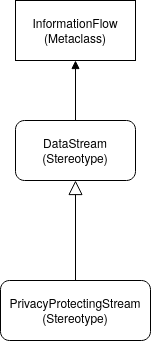
\includegraphics[scale=0.3]{./chapter4/umlProfile/PrivacyProtectingStreamUMLProfile.png}}
\caption{PrivacyProtectingStream UML Profile}
\label{fig:PrivacyProtectingStream UML Profile}
\end{figure}

\subsection{PrivacyPolicyPackage}

StreamGen uses a package called StreamDatatypes in order to collect all the DataTypes that are flowing through the streams. The DataTypes that are specified inside the package allow the users to specify the different values that are conveyed in a stream but inside the same tuple. Following these approach, a new package called PrivacyPolicyPackage has been added to the UML profile in order to collect all the sources involved in the privacy policies applications, SCV sources and user privacy policies.

These sources are not going to be connected directly to the streams or to the transformations of the DIA but they are going to allow the users to specify from where the different variables required to protected the streams are taken. As they are not going to be connected, a package to put all of them together is added to the language.

In the figure \ref{fig:PrivacyPolicyPackage UML Profile} can be seen the UML profile of this package.

\begin{figure}
\centering
{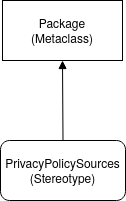
\includegraphics[scale=0.3]{./chapter4/umlProfile/PrivacyPolicyPackageUMLProfile.png}}
\caption{PrivacyPolicyPackage UML Profile}
\label{fig:PrivacyPolicyPackage UML Profile}
\end{figure}


\subsubsection{PrivacyContextSource}

Static Context Variables are required in order to know when an user specified privacy policy can be apply. These SCVs can be just an agent or many of them. This is why a wide variety of possibilities have been developeded in order to allow the users to choose the most appropriate SCV source. Such possibilities are:

\begin{itemize}
\item PrivContTextFileSource.
\item PrivContSocketSource.
\item PrivContKafkaSource.
\item PrivContFixedSource.
\end{itemize}

Following the approach of StreamGen with DataSource, a stereotype called PrivacyContextSource has been created as a generalization of the already existing DataSource stereotype. This new stereotype have four generalizations, the four possibilities to choose by the user when the SCV source has to be defined. Each of these four sources have its own properties. These properties have been defined taking into account the already existing data sources:

\begin{itemize}
\item TextFileSource.
\item SocketSource.
\item KafkaSource.
\end{itemize}

TextFileSource stereotype reads a file which contains all the input values of the DIA. When the user selects the stereotype,the path (pathToFile) from where the DIA must read the file has to be specified. PrivContTextFileSource works exactly in the same way, this stereotype contains a property called pathToFile (String) where the user will have to specify the path where the file with all the SCV tuples is located. SocketSource stereotype is connected to a port and to a host by means of the properties host (String) and port (Integer) that the user specifies when the stereotype is defined. Following this approach, PrivContSocketSource is connected by a port (Integer) and a host (String) to a server which supplies the SCV tuples.Finally, the KafkaSource is connected by means of kafkaBrokerIp (String) and kafkaBrokerPort (Integer) to a Kafka server. PrivContKafkaSource connects a DIA to a Kafka server that provides the SCV tuples by means of two properties as in the case of the KafkaSource.

In case of PrivContTextFileSource and PrivContSocketSource, when the code is generated a NonParallelStream called contextString which contains the SCV tuples (Strings) is introduced into the DIA. This stream is automatically sent to a map transformation which is imported from the library. This map transformation parses contextString to a stream composed with the DataType specified by the user. This DataType should contain the same data that each of the strings but the values are split by the comma in order to have each of the values independently. Moreover, this stream is called contextStream and it will be used to apply the privacy policies.

Finally, PrivContFixedSource is a source imported from the library which allows the users to specify only one SCV source. In order to do this, when the user is defining the UML model of the DIA, three properties must be specified. This three properties are fixedUser (String), fixedRole (String) and fixesPuporse (String) which allow to specify the static or fixed SCV source.

In case of PrivContKafkaSource and PrivContFixedSource the contextStream with the user specified DataType is directly generated without applying any transformation.

\subsubsection{PrivacyPolicySource}

In addition to SCVs, StreamGen requires some user specified rules to guarantee privacy. These rules are going to be written in a YAML file that must be imported to the DIA in order to feed the privacy library. In order to do this, the library snakeyaml (org.yaml.snakeyaml.Yaml) is used. This is the unique type of sources for such purpose as the rules are supposed to be stored in a YAML file.

Following the approach of DataSource stereotype, a new stereotype called PrivacyPolicySource is created as a generalization of the DataSource stereotype. The goal with this stereotype is to have the possibility to add different type of sources as currently is happening with the SCV source. From the PrivacyPolicySource stereotype, a new generalization is created in order to make the relationship with a new stereotype called PrivPolYamlFileSource. This stereotype represents the insertion of the YAML file to the DIA. In order to specify the path where the YAML file is located, a new property (pathToFile, String) is added to the stereotype. With this property, the user is able to define the location where the file is stored and from where the DIA must read the privacy policy rules written by the user.

In the figure \ref{fig:PrivacyPolicyDataSources Classes UML Profile} can be seen the language of the PrivacyContextSource and PrivacyPolicySource represented in a UML profile diagram.

\begin{figure}
\centering
{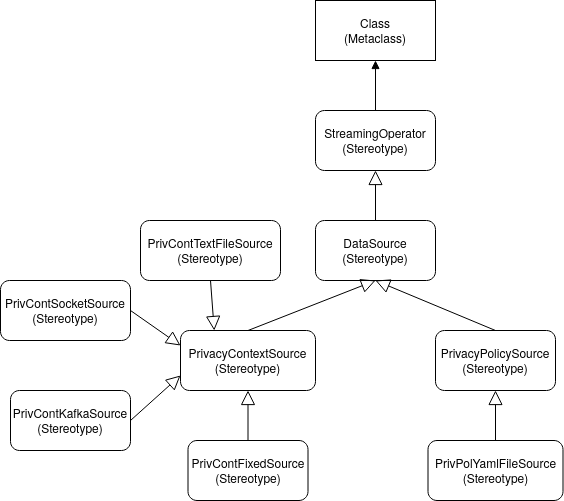
\includegraphics[scale=0.3]{./chapter4/umlProfile/PrivacyPolicyDataSourceUMLProfile.png}}
\caption{PrivacyPolicyDataSources Classes UML Profile}
\label{fig:PrivacyPolicyDataSources Classes UML Profile}
\end{figure}

\section{Privacy Policy Translation}

The UML metamodel that specifies the language for the privacy policies must be by the user in order to create the UML class diagram of the DIA. This diagram is used by Acceleo in order to generate the final code which runs in Flink. In this section this step is explained. Furthermore, all along this section an assumption is taken. This assumption is that the UML file generated by Papyrus is going to contain all the packaged classes in the following order:

\begin{enumerate}
\item Sources.
\item Transformations.
\item Sinks.
\end{enumerate}

First of all, all the sources introducing data are going to be packaged as elements in the UML file that is generated by Papyrus. After them, all the transformations are packaged. Finally, all the sinks where the data must be stored are packaged. This assumption is similar to say that the DIA is built in order without adding transformations, sinks or sources after generating the DIA. This is important in order to generate a target code in order and without modifications of pieces of code once it has already been generated.

In addition to this assumption, the target code generated by means of StreamGen must be able to follow a structure that will generate the same pieces of code from the UML language.

\subsection{Privacy Policy Codes Structure}

The generated codes when the designed DIA must be privacy policy aware must follow a predefined structure in order to use correctly the privacy policy libraries used in \cite{privacypoliciesarticle}. This structure is going to have four parts:

\begin{enumerate}
\item Library Import.
\item Privacy Policy Initialization.
\item Streams Declaration.
\item Streams Protection.
\end{enumerate}

\subsubsection{Library Import}

First of all  a condition is required in order to import the libraries of \cite{privacypoliciesarticle} only when they are required. Then, libraries are going to be imported when in the application model exists at least one PrivacyProtectingStream stereotype. If the DIA is not privacy policy aware, there is no PrivacyProtectingStream stereotype and the different libraries are not imported. The imported libraries are:

\begin{itemize}
\item import org.apache.commons.io.FileUtils;
\item import java.io.File;
\item import org.yaml.snakeyaml.Yaml;
\item import it.deib.polimi.diaprivacy.library.GeneralizationFunction;
\item import it.deib.polimi.diaprivacy.library.ProtectedStream;
\item import it.deib.polimi.diaprivacy.model.ApplicationDataStream;
\item import it.deib.polimi.diaprivacy.model.ApplicationPrivacy;
\item import it.deib.polimi.diaprivacy.model.DSEP;
\item import it.deib.polimi.diaprivacy.model.PrivacyContext;
\item import it.deib.polimi.diaprivacy.library.PrivacyContextParser;
\item import it.deib.polimi.diaprivacy.model.VCP;
\item import it.deib.polimi.diaprivacy.library.PrivacyContextFixedSource;
\end{itemize}

The library it.deib.polimi.diaprivacy.library can be found in the repository \url{https://github.com/MicheleGuerriero/dataflow-privacy-library/tree/master/src/main/java/it/deib/polimi/diaprivacy/library}.

And the library it.deib.polimi.diaprivacy.model can be found in the repository \url{https://github.com/MicheleGuerriero/common/tree/master/src/main/java/it/deib/polimi/diaprivacy/model}.

Finally, the org.yaml.snakeyaml.Yaml library must be imported from the POM file. In order to do this, in the POM file generation Acceleo file (generateFlinkPom.mtl), a dependency is triggled when a PrivacyProtectingStream exists in the application model.

\subsubsection{Privacy Policy Initialization}

At this part, StreamGen is going to extract the information supplied by the user in the PrivacyPolicySources package. In order to do this, each of the packages contained in the application model are taken and if the package is the PrivacyPolicySources, for each of the classes contained in the package a different action is applied taking into account the class type. In the table \ref{Applied Actions for Class Stereotypes in PrivacyPolicySources Package} each of the rows represent: for each class stereotype that can be contained in the PrivacyPolicySources package, the action that will be applied.

\begin{table}[h!]
\centering
	\begin{tabular}{||c|c||} 
	\hline\hline
	Class Stereotype & Applied Action \\ [1ex] 
	\hline\hline
	PrivPolYamlFileSource & generateFlinkPrivacyPolicyYamlFileSource  \\
	\hline
	PrivContFixedSource & generateFlinkPrivacyContextFixedSource  \\
	\hline
	PrivContKafkaSource & generateFlinkPrivacyContextKafkaSource  \\
	\hline
	PrivContTextFileSource & generateFlinkPrivacyContextTextFileSource  \\
	\hline
	PrivContSocketSource & generateFlinkPrivacyContextSocketSource  \\
	\hline\hline
	\end{tabular}
\caption{Applied Actions for Class Stereotypes in PrivacyPolicySources Package}
\label{Applied Actions for Class Stereotypes in PrivacyPolicySources Package}
\end{table}

All the actions that must be applied when there is any of the class stereotypes specified in the table \ref{Applied Actions for Class Stereotypes in PrivacyPolicySources Package} are written in the generateFlinkSources.mtl file of the StreamGen Acceleo project as public templates.

In the figures \ref{fig:GenerateFlinkPrivacyPolicyYamlFileSource Acceleo Template} and \ref{fig:GenerateFlinkPrivacyContextTextFileSource Acceleo Template} can be seen the examples of such generation actions for the class stereotypes PrivPolYamlFileSource and PrivContTextFileSource.

\begin{figure}
\centering
{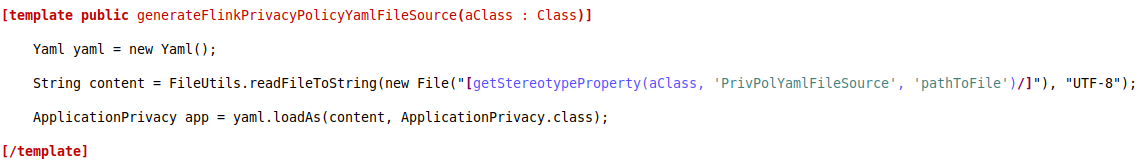
\includegraphics[scale=0.3]{./chapter4/codeStructure/GenerateFlinkPrivacyPolicyYamlFileSource.png}}
\caption{GenerateFlinkPrivacyPolicyYamlFileSource Acceleo Template}
\label{fig:GenerateFlinkPrivacyPolicyYamlFileSource Acceleo Template}
\end{figure}

\begin{figure}
\centering
{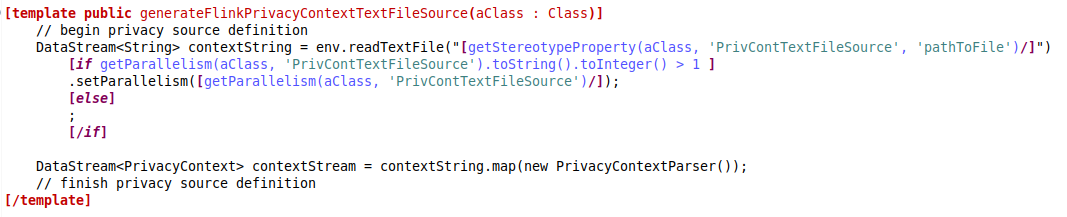
\includegraphics[scale=0.3]{./chapter4/codeStructure/GenerateFlinkPrivacyContextTextFileSource.png}}
\caption{GenerateFlinkPrivacyContextTextFileSource Acceleo Template}
\label{fig:GenerateFlinkPrivacyContextTextFileSource Acceleo Template}
\end{figure}

\subsubsection{Streams Declaration}

After generating and parsing the SCVs and the privacy policy YAML file in the Privacy Policy Initialization part, StreamGen is going to declare all those streams that are introduced to a transformation and that the PrivacyProtectingStream stereotype is not applied on them. In order to do this, another condition must be taken into account as any stream of a DIA which is not privacy policy aware satisfies the condition and, in that case, the streams must not be declared.

Thus, any time that a transformation is generated, after generating the piece of code corresponding to the transformation, two conditions are taken into account. The first condition checks that the input stream of the transformation is not a PrivacyProtectingStream. The second condition checks that exists at least one PrivacyProtectingStream stereotype in the application model. If both conditions are satisfied then the stream is set into the privacy policy YAML file.
